%!TEX root=../../../main.tex

The concrete implementation of the basic annotation model presented in
Subsection \ref{sec:anno} consists of a JSON representation similar to the one
in Fig. \ref{lst:basejson}.

\begin{figure}[!ht]
  \lstinputlisting[frame=tb,
                   captionpos=b,
                   basicstyle=\ttfamily,
                   numbers=none,
                   showspaces=false,
                   showstringspaces=false,
                   showtabs=false,
                   stepnumber=2,
                   numbersep=4pt]
    {static/lst/base.json}
  \caption[Base JSON model for annotations]
          {Base JSON model for annotations; each field is denoted by its name
           and held data type.}
  \label{lst:basejson}
\end{figure}

Each annotation should be distinguished by a Universally Unique Identifier
(UUID) and have its target associated either explicitly or implicitly (through
application specific translations) with an IRI. Other fields include the author
of the annotation (an Invenio user), its textual body, time stamp, and access
restrictions.

This model facilitated the implementation of an annotation system which allows
adding metadata on any Web page of Invenio; users can add such annotations by
using a dialog similar to the one in Fig. \ref{fig:annoform}.

\begin{figure}
  \centering
  \fbox{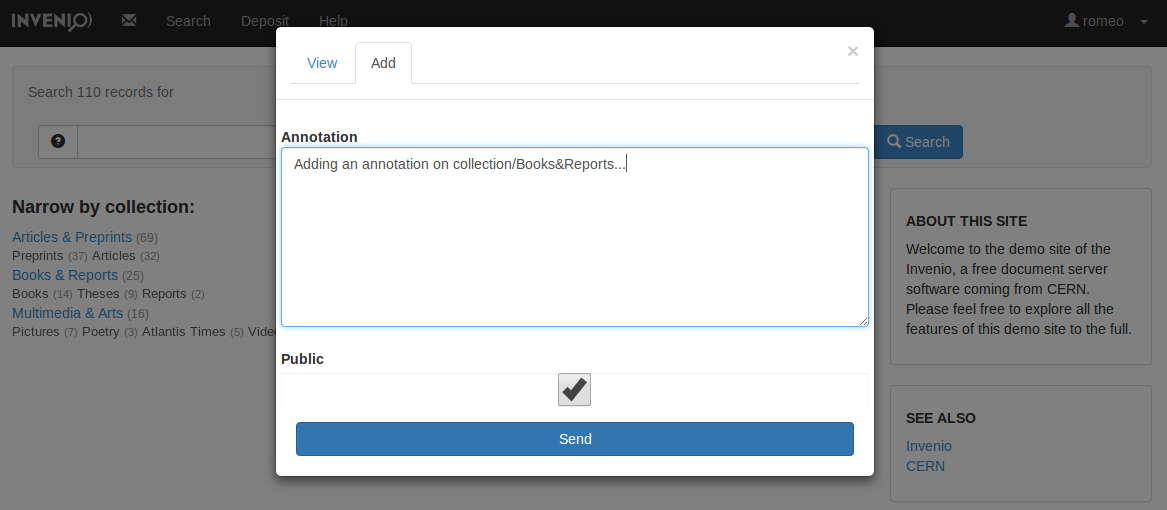
\includegraphics[scale=0.395]{static/img/annoform.png}}
  \caption[Form allowing to add annotations on any Invenio page]
          {Form allowing to add annotations on any Invenio page. Users can add
           add a textual body and specify if the annotation should be public,
           visible to any Web page visitor, or private, visible only to them.}
  \label{fig:annoform}
\end{figure}

The communication between the frontend interface and backend system is mediated
by view functions defined in so-called Flask blueprints. Apart from allowing
users to input data, displaying annotations is also possible.

Annotations are stored in a MongoDB database \cite{ref:mongo} using the
facilities provided by JSONAlchemy. This module allows defining a schema for
JSON documents, in which the collection of fields and various restrictions on
them can be defined; for example, the UUID is required for all annotations, and
the time stamp should have a standard format. Moreover, JSONAlchemy allows
querying the stored objects (e.g., get all annotations with the target being
the main page of CDS), and modifying them. A thin wrapper for adapting these
operations to the annotation use case is included in an internal API, which can
be used by the Flask blueprint, REST interface (see Subsection \ref{sec:pub}),
or even other Invenio modules to access annotation data. An overview of the
workflow is included in Fig. \ref{fig:baseanno}.

\begin{figure}
  \centering
  \fbox{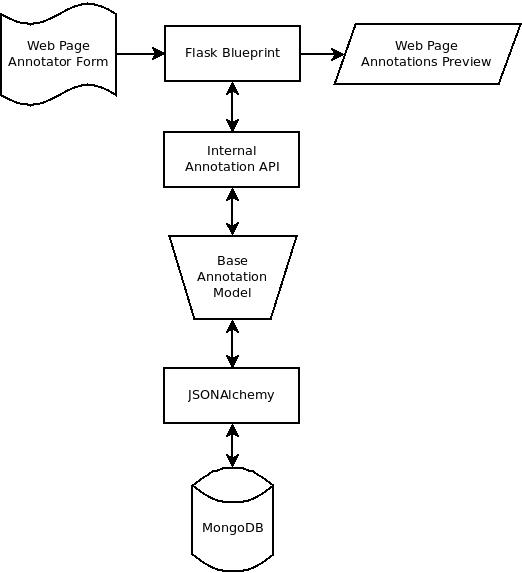
\includegraphics[scale=0.6]{static/dia/base_anno.jpeg}}
  \caption[Web page annotation workflow]
          {Web page annotation workflow; users can add annotations on any
           IRI-identified resource. The specialised API stores data in a
           MongoDB database using the JSONAlchemy model. The Flask blueprint
           provides both annotation creation and display facilities to users
           through its views.}
  \label{fig:baseanno}
\end{figure}
